% =====================================================================
%  deck_week.tex  --  meeting deck, 2026-09 (beamer, 16:9)
%
%  Shape (2026-09-18, Ray's direction): a thesis presentation, not a
%  progress report. Part I is the thesis so far (problem, model in four
%  method frames lifted from the July lab talk, one status frame per
%  phase); Part II is the two measured weeks in their place inside that
%  arc; then the asks and the backups. Fundamentals are IN the deck so
%  Phase-1 work and model basics can be revisited in the room.
%
%  Style: house rules from the July lab talk. No em-dashes, no
%  semicolons, no asterisks on slides ("significant", never "starred").
%  One term per concept. Symbols defined with role and units. Only show
%  what is used. Never say bare "AR(1)" in the room: say "correlated
%  timing noise across notes".
%
%  Every number traces to a results/ doc or the thesis draft. All new
%  results are development level, exploratory, published tables
%  unchanged.
%
%  Compile:  cd docs/slides && tectonic deck_week.tex
% =====================================================================
\documentclass[aspectratio=169,11pt]{beamer}
\usetheme{default}
\usefonttheme{professionalfonts}
\setbeamertemplate{navigation symbols}{}
\setbeamertemplate{itemize items}{\textcolor{okblue}{\scriptsize$\blacksquare$}}
\setbeamertemplate{footline}{%
  \hfill\scriptsize\textcolor{muted}{\insertframenumber\,/\,\inserttotalframenumber}\hspace{2mm}\vspace{2mm}}

\usepackage{amsmath,amssymb,bm}
\usepackage{booktabs}
\usepackage{graphicx}
\graphicspath{{../thesis/figures/}}

\definecolor{okblue}{HTML}{0072B2}
\definecolor{okverm}{HTML}{D55E00}
\definecolor{okgreen}{HTML}{009E73}
\definecolor{okamber}{HTML}{E69F00}
\definecolor{muted}{HTML}{6B7280}
\definecolor{ink}{HTML}{1A1A1A}
\setbeamercolor{frametitle}{fg=ink}
\setbeamercolor{normal text}{fg=ink}
\setbeamerfont{frametitle}{series=\bfseries,size=\large}

\newcommand{\figslotw}[3]{%
  \begin{center}
  \includegraphics[width=#2\textwidth]{#1}
  \end{center}}

\newcommand{\R}{\mathbb{R}}
\newcommand{\N}{\mathcal{N}}
\newcommand{\Lg}{L_{\mathcal G}}
\newcommand{\diag}{\operatorname{diag}}

\title{\textbf{Expressive Performance as a Gaussian Process\\ on a Musical Score Graph}}
\subtitle{The thesis so far, and two weeks of measured answers}
\author{Raynaldi Lalang}
\institute{Kyoto University}
\date{September 2026}

\begin{document}

% ---------------------------------------------------------------------
\begin{frame}
  \titlepage
\end{frame}

% ============================================== PART I  THE THESIS
% ---------------------------------------------------------------------
\begin{frame}{Problem: infer how the music was played, with reliable uncertainty}
  The goal: a probabilistic model of \textbf{every per-note expressive
  parameter a performer controls}: timing, articulation, velocity, and, on
  continuously pitched instruments, intonation and vibrato, ultimately
  inferred from audio alone. Every estimate must carry an error bar that can
  be trusted note by note.
  \vspace{2mm}

  On piano, from aligned performance MIDI,
  \begin{equation*}
    y_i \;=\; \bigl[\;\underbrace{\tau_i}_{\text{onset timing}},\;\;
      \underbrace{\log r_i}_{\text{articulation}},\;\;
      \underbrace{v_i}_{\text{velocity}}\;\bigr] \in \R^{3}
    \qquad\text{per written note.}
  \end{equation*}
  \begin{itemize}
    \item Not full transcription: the score is known.
    \item The output is a \textbf{per-note posterior}: an estimate and a
          calibrated error bar.
    \item On strings and winds the vector extends to six estimated
          channels (Phase 2).
  \end{itemize}
\end{frame}

% ---------------------------------------------------------------------
\begin{frame}{Approach: one prior, three kinds of observation}
  One \textbf{Gaussian process (GP)} prior over per-note expressive fields, on
  a graph built from the score. Only the observation changes: per-note MIDI
  values (Phase 1), noisy $f_0$-derived targets (Phase 2), or the waveform
  itself (Phase 3). A Phase-0 music model supplies input features to all.
  \figslotw{deck_programme.png}{0.9}{the shared prior with three swappable
    likelihood blocks (MIDI / $f_0$ / waveform)}
\end{frame}

% ---------------------------------------------------------------------
\begin{frame}{The model (1): the score graph}
  Nodes are the $N$ written notes: pitch $p_i$, beat onset $b_i$, beat
  duration $d_i$. Edges connect notes close in score time and pitch
  (neighbours should be played similarly):
  \vspace{-1mm}
  \begin{equation*}
    W_{ij} \;=\; \exp\!\Bigl( -\tfrac{(b_i - b_j)^2}{2\,\ell_b^2}
                             \;-\; \tfrac{(p_i - p_j)^2}{2\,\ell_p^2} \Bigr),
    \qquad
    \Lg \;=\; D - W .
  \end{equation*}
  \vspace{-2mm}
  {\centering\small $\ell_b, \ell_p$: length-scales. $D_{ii} = \sum_j W_{ij}$.
  $\Lg$: the graph Laplacian. $W, D, \Lg \in \R^{N \times N}$.\par}
  \figslotw{deck_scoregraph.png}{0.80}{a few bars of real score as nodes,
    edges drawn by time / pitch / chord relation}
\end{frame}

% ---------------------------------------------------------------------
\begin{frame}{The model (2): a GP on the graph, channels coupled}
  Eigendecompose the Laplacian, $\Lg = U \diag(\nu)\, U^{\!\top}$
  ($U \in \R^{N \times N}$ eigenvectors, $\nu \in \R^N$ eigenvalues), and
  shape its spectrum with one parameter $s$:
  \begin{equation*}
    K_G(s) \;=\; U\, g(\nu; s)\, U^{\!\top},
    \qquad
    g(\nu; s) \;=\; \frac{1}{1 + s\,\nu}
    \quad\text{(graph Mat\'ern, } \alpha = 1\text{)} .
  \end{equation*}
  Smooth-on-the-graph components keep their variance, rough ones are shrunk.
  \vspace{1mm}

  The channels are correlated, so they share the graph through a learned
  coupling matrix $B$ ($c, c'$ index the channels):
  \begin{equation*}
    \operatorname{Cov}\bigl[\, y_{i,c},\; y_{j,c'} \bigr]
      \;=\; B_{cc'}\, \bigl[K_G(s)\bigr]_{ij}
    \qquad\Longleftrightarrow\qquad
    \operatorname{Cov}[\,y\,] \;=\; B \otimes K_G(s).
  \end{equation*}
  An observed channel at one note then informs the other channels at
  neighbouring notes.
\end{frame}

% ---------------------------------------------------------------------
\begin{frame}{The model (3): side information as kernels}
  Any per-note side information enters the same way. In Phase 1 there are
  two sets, each one row per note ($N \times d$): simple score descriptors
  $X_{\mathrm{feat}}$ (register, duration, meter, position) and per-note
  features $H$ from a small music model trained on MAESTRO.
  \vspace{1mm}

  A linear mean with unknown weights $\beta$, integrated out, becomes a
  kernel term ($X$ = either feature matrix, $f_G$ = the graph GP of the
  previous slide, $c_X$ = the prior scale of set $X$'s weights):
  \begin{equation*}
    y \;=\; X\beta + f_G, \quad \beta \sim \N(0,\, c_X\,I)
    \qquad\Longrightarrow\qquad
    \operatorname{Cov}[\,y\,] \;=\; c_X\, X X^{\!\top} + \operatorname{Cov}[\,f_G\,].
  \end{equation*}
  \begin{itemize}
    \item So the regression weights are not fixed once across the corpus: they
          are \textbf{re-inferred for every piece}, jointly with everything
          else, and their uncertainty enters the posterior.
    \item This per-piece adaptation is the measured main source of the
          accuracy gain.
  \end{itemize}
\end{frame}

% ---------------------------------------------------------------------
\begin{frame}{The model (4): the covariance of one performance}
  Stack all channels of the $N$ notes into one vector $y$.
  Every component becomes one term of its covariance $K$, built per piece:
  \begin{equation*}
    K \;=\;
    \underbrace{\textcolor{okblue}{B \otimes K_G(s)}}_{\text{coupled graph GP}}
    \;+\; \underbrace{\textcolor{okamber}{\textstyle\sum_f \diag(c_f)\otimes X_f X_f^{\!\top}}}_{\text{side information}}
    \;+\; \underbrace{\textcolor{okverm}{\diag(\varsigma^2)\otimes I}}_{\text{noise}}
  \end{equation*}
  {\small $f$ runs over the feature sets, giving per-channel scales $c_f$.
  $\varsigma^2$ = the per-channel noise variances.}
  \vspace{1mm}

  All parameters $\theta = (s, B, \{c_f\}, \varsigma^2)$, 16 numbers in
  Phase 1, from one exact evidence per piece. Prediction is conjugate:
  \begin{equation*}
    m = C_{\cdot o} K_{oo}^{-1} \tilde y_o, \qquad
    \Sigma_y = C - C_{\cdot o} K_{oo}^{-1} C_{o\cdot},
  \end{equation*}
  {\small $\tilde y_o$: the observed values. $o$: the observed entries of
  $y$. $C$: the noise-free part of $K$. $m, \Sigma_y$: posterior mean and
  covariance. No variational approximation anywhere, and the baselines are
  exact special cases (diagonal $B$, zero $c_f$, fixed cross-piece mean).
  Today's main result adds one parameter to the
  \textcolor{okverm}{noise term}.}
\end{frame}

% ---------------------------------------------------------------------
\begin{frame}{Phase 1 (piano, ASAP): \textcolor{okgreen}{confirmed}}
  Preregistered one shot on 20 untouched pieces, against the two stage
  pipeline the model provably contains:
  \begin{itemize}
    \item \textbf{Accuracy}: RMSE 0.376 vs 0.393, paired difference
          significant.
    \item \textbf{Calibration}: the graph's log score contribution
          significant, coverage 0.925 at nominal 0.9.
    \item \textbf{Attribution} (measured): the per-piece feature weighting
          carries the mean, the graph carries the calibration, and the
          two components are near-orthogonal complements.
  \end{itemize}
  \vfill
  Known boundary: per-piece adaptation fails at excerpt extrapolation
  (completion), where the cross-piece head stays the honest tool. One
  documented wart: a rare timing-outlier tail can explode the pooled
  Gaussian log score on very steady pieces (measured fix today).
\end{frame}

% ---------------------------------------------------------------------
\begin{frame}{Phase 2 (strings and winds, URMP): \textcolor{okgreen}{confirmed}, one claim failed}
  The same prior, unchanged. Six per-note channels estimated from audio,
  each with its own variance, used as given:
  \begin{equation*}
    y_i = [\, c_i,\ \log\gamma_i,\ \log f_i,\ \ell_i,\ \tau_i,\ d_i^{\mathrm{vib}} \,]
    \quad
    \text{\small (intonation, extent, rate, loudness, timing, vibrato onset)}
  \end{equation*}
  Registered claims, one shot spent 2026-08-27, scored by the frozen rule:
  \begin{itemize}
    \item \textcolor{okgreen}{C1 pass}: intonation recovery ($-0.877$,
          significant, reproducing development).
    \item \textcolor{okgreen}{C2 pass}: vibrato calibration, both channels.
    \item \textcolor{okgreen}{C3 pass}: coverage 0.88 to 0.91 on all six
          channels.
    \item \textcolor{okverm}{C4 fail}: timing calibration ($-0.030$, not
          significant), reported verbatim. The thesis names the suspect:
          alignment error correlated along score time.
  \end{itemize}
  \vfill
  The failed claim is where today's main result attaches.
\end{frame}

% ---------------------------------------------------------------------
\begin{frame}{Phase 3 (waveform likelihood): scoped, first studies measured}
  The likelihood block becomes the audio itself: a synthesis basis with the
  amplitudes marginalized exactly, so pitch deviations are scored directly
  against the waveform.
  \begin{itemize}
    \item \textbf{Feasibility} (376 notes, 7 tracks): waveform intonation
          lands median 2.29 cents from quasi-truth with \textbf{no pitch
          tracker}, and beats the estimator chain on winds.
    \item \textbf{Integration}: as a seventh bundle channel with a
          visible-notes discrepancy floor, better calibrated on 14 of 14
          pairs (significant). The no-floor control is worse, so the floor
          is necessary.
    \item \textbf{Open}: joint inference over note positions.
  \end{itemize}
  \vfill
  {\small\textcolor{muted}{All Phase 3 numbers are development studies, no
  claims. Record: results/phase3\_waveform\_dev.md and
  results/phase3\_integration\_dev.md.}}
\end{frame}

% ============================================== PART II  THE TWO WEEKS
% ---------------------------------------------------------------------
\begin{frame}{Since we last met}
  \begin{enumerate}
    \item \textbf{Last meeting} was the reading week: the two kernel
          pointers from our discussion, the three papers, and the two
          slots where those kernels could enter our pipeline.
    \item \textbf{Then the estimator test we agreed on}: the swap was
          closed by its pre committed rule. The model itself won at curve
          level, both sides on the next slide.
    \item \textbf{Then a measuring week}: the second slot and a learned
          filter closed the kernel question, and every limitation the
          thesis had documented about itself was measured. Results
          hardened (a multiple comparison pass, three run reproduction),
          winners adopted as opt in machinery, one registration drafted.
  \end{enumerate}
  \vfill
  {\small\textcolor{muted}{I measured instead of building. Everything is
  development level, published tables unchanged. Ledger:
  results/exploration\_week\_2026-09.md. Every significance claim on
  these slides survives the multiple comparison pass.}}
\end{frame}

% ---------------------------------------------------------------------
\begin{frame}{The kernel direction: measured at both slots}
  \begin{enumerate}
    \item \textbf{As a model of the curve, it wins.} Scored frame by
          frame against the ground truth pitch curves, the spectral
          mixture GP describes what the player did better than the
          sinusoid (median 6.3 vs 9.6 cents).
    \item \textbf{As a drop in for the current estimator, it loses.}
          Our channels are the sine fit's own parameters. Translating a
          posterior over curves into those three scalars is less stable
          than never leaving them (pre committed rule, verified intrinsic
          on strongly vibrated notes). The confirmed bundle keeps its
          estimator.
    \item \textbf{The same pattern at the other slot and for a learned
          filter}: no gain as the waveform curve prior at matched rank,
          and a free spectral bump is switched off by the evidence on 90
          percent of pieces.
  \end{enumerate}
  \vfill
  The reading: the model may have outgrown the scalar interface, not the
  other way round. What it already changed: curve level scoring, a
  coherence bound, and the realized quantities read out rule.
\end{frame}

% ---------------------------------------------------------------------
\begin{frame}{The timing tail: fixed at both levels}
  Known Phase 1 failure: on a very steady piece a few timing outliers
  explode the pooled Gaussian log score.
  \begin{itemize}
    \item \textbf{Deploy time.} A variance matched Student t predictive
          takes the documented blow up cell from 105.2 to $-1.7$ with
          coverage intact. The predictive floor we had suggested does
          nothing: this is a tail shape problem, not a scale problem.
    \item \textbf{Inference level.} Fitting the timing noise as a
          Student t (scale mixture, leave one out reweighting) brings
          coverage to nominal and improves \textbf{articulation} recovery
          by $-0.018$ (significant): an observed timing outlier corrupts
          the coupled channels, and only robustifying the fit undoes that.
  \end{itemize}
\end{frame}

% ---------------------------------------------------------------------
\begin{frame}{The failed confirmation claim now has a measured fix}
  C4 (timing calibration) failed at the Phase 2 confirmation. The thesis
  named the suspect: alignment error is correlated along score time, and
  a diagonal noise row cannot represent it.
  \[ \Sigma^{\tau}_{ij} = \sqrt{d_i d_j}\; \rho^{|i-j|}
     \qquad (d_i = \text{the note's timing noise variance, } i, j
     \text{ in score order}) \]
  \begin{itemize}
    \item One correlation parameter $\rho$ in the timing noise row,
          chosen per piece by the evidence itself.
    \item The evidence detects the correlation on 97 to 100 percent of
          pieces (median 0.45 to 0.60).
    \item Timing calibration improves ($\Delta$NLL $-0.111$, significant),
          coverage moves to nominal, and timing error falls about
          20 percent (99 to 80 ms).
    \item Reproduced three ways: original masks, fresh masks, and a full
          joint refit.
  \end{itemize}
\end{frame}

% ---------------------------------------------------------------------
\begin{frame}{The same result, in one picture}
  \centering
  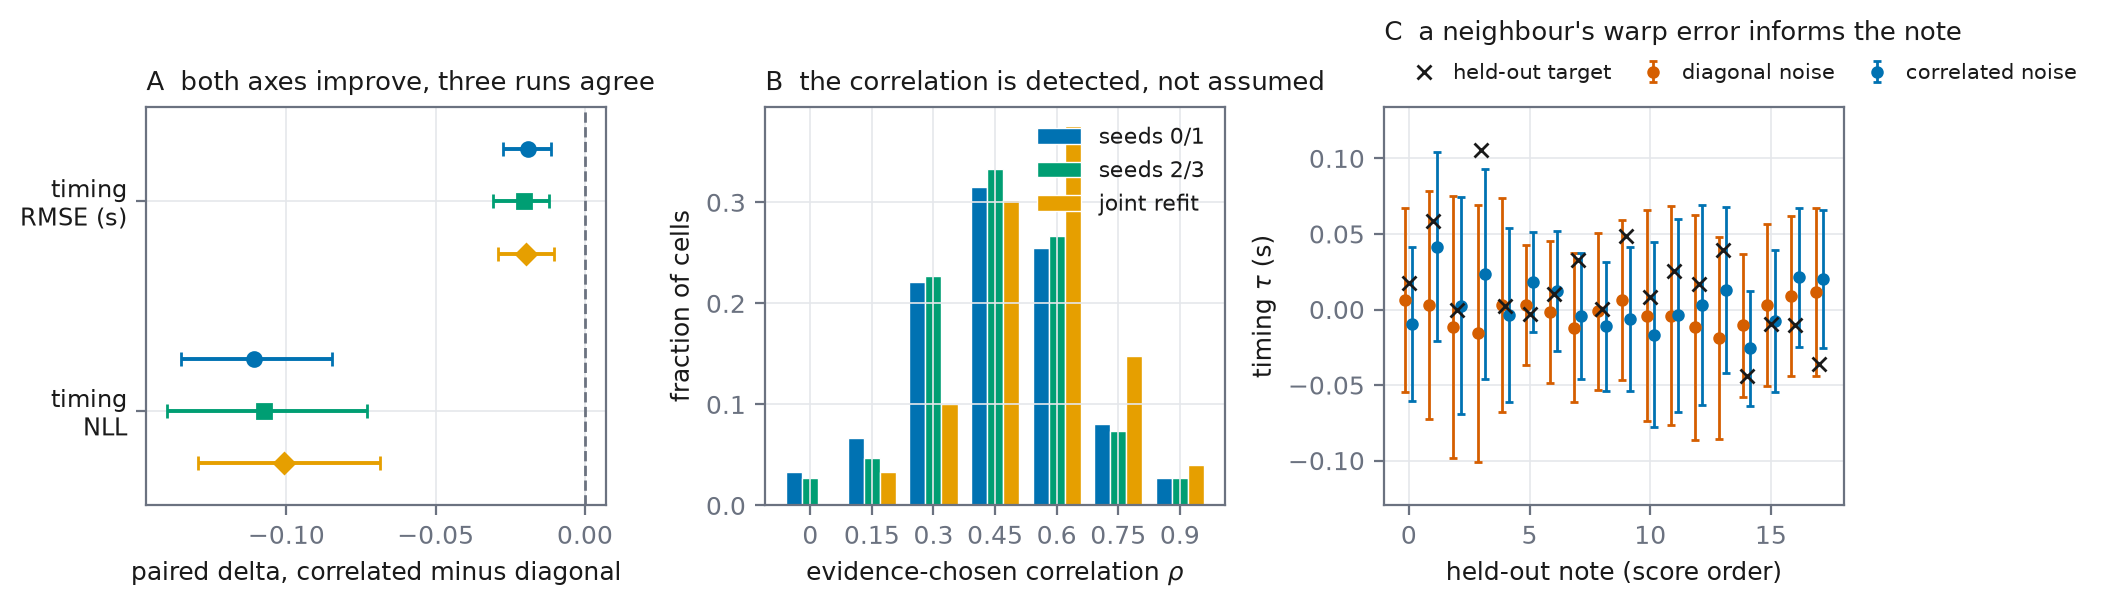
\includegraphics[width=0.98\linewidth]{corrnoise_tau_dev.png}

  {\scriptsize\textcolor{muted}{Left: paired deltas with 95 percent
  intervals, three runs. Middle: the evidence-chosen correlation per
  piece. Right: one track's held-out timing, diagonal vs correlated
  noise, targets as crosses.}}
\end{frame}

% ---------------------------------------------------------------------
\begin{frame}{The registration is drafted. It needs one decision.}
  \centering
  \begin{tabular}{@{}rcc@{}}
    \toprule
    pool size (pieces) & P(calibration claim significant) & P(recovery claim significant) \\
    \midrule
     6 & 0.99 & 0.76 \\
    10 (Bach10 size) & 1.00 & 0.83 \\
    13 (spent pool size) & 1.00 & 0.94 \\
    15 & 1.00 & 0.99 \\
    \bottomrule
  \end{tabular}
  \vfill
  \begin{itemize}
    \item Claims ordered by this table: calibration primary, recovery
          secondary. Draft: docs/corrnoise\_prereg\_DRAFT.md.
    \item URMP is fully spent, so the pool must be a new corpus, a
          disclosed re use, or both. The tonal metric registration waits
          on the same decision.
  \end{itemize}
\end{frame}

% ---------------------------------------------------------------------
\begin{frame}{What I would like from you today}
  Everything above is implemented as opt in capabilities: default off,
  published paths bit unchanged, pinned by equality tests.
  \begin{enumerate}
    \item \textbf{The pool decision} for the correlated timing noise
          registration (and the tonal one): new corpus such as Bach10,
          disclosed re use of the spent URMP pool, or both.
    \item \textbf{The adoption defaults}: are you comfortable with the
          robust timing noise, the correlated timing noise, and the
          completion guard as recommended opt in modes for new runs?
    \item \textbf{The kernels are your call.} They won at curve level
          and lost at impersonating the sine fit's parameters. Three
          paths: marginalize the rate and retest the estimator, aim the
          kernels at curve level channels inside Phase 3, or close and
          spend the next cycle on the timing registration. My default is
          the last now and the second eventually.
  \end{enumerate}
  \vfill
  {\small\textcolor{muted}{Everything else is recorded and waiting:
  seven results documents, the ledger, the updated draft (71 pages), and
  the registration draft.}}
\end{frame}


% ------------------------------------------------------------ backup
\begin{frame}{Backup: the estimator on one real note (the win side)}
  \centering
  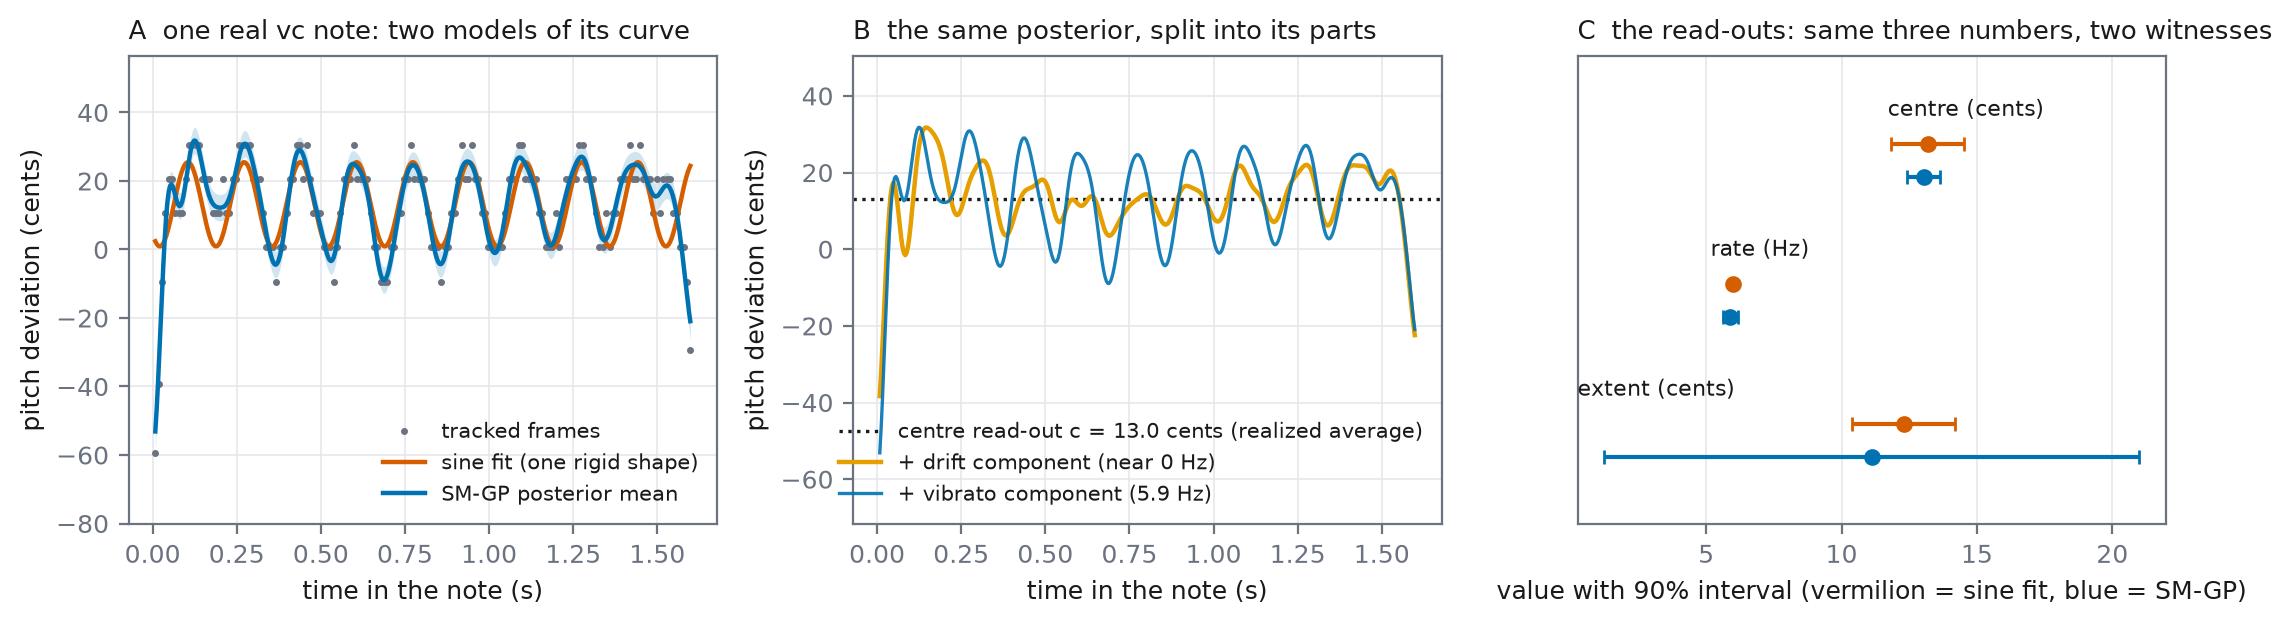
\includegraphics[width=0.98\linewidth]{sm_estimator_explainer.png}

  {\scriptsize\textcolor{muted}{One cello note. A: the sine fit's rigid
  shape drifts out of phase, the SM GP tracks the curve. B: the posterior
  split into centre, drift, and vibrato. C: both estimators' read outs.}}
\end{frame}

\begin{frame}{Backup: the estimator on one real note (the loss side)}
  \centering
  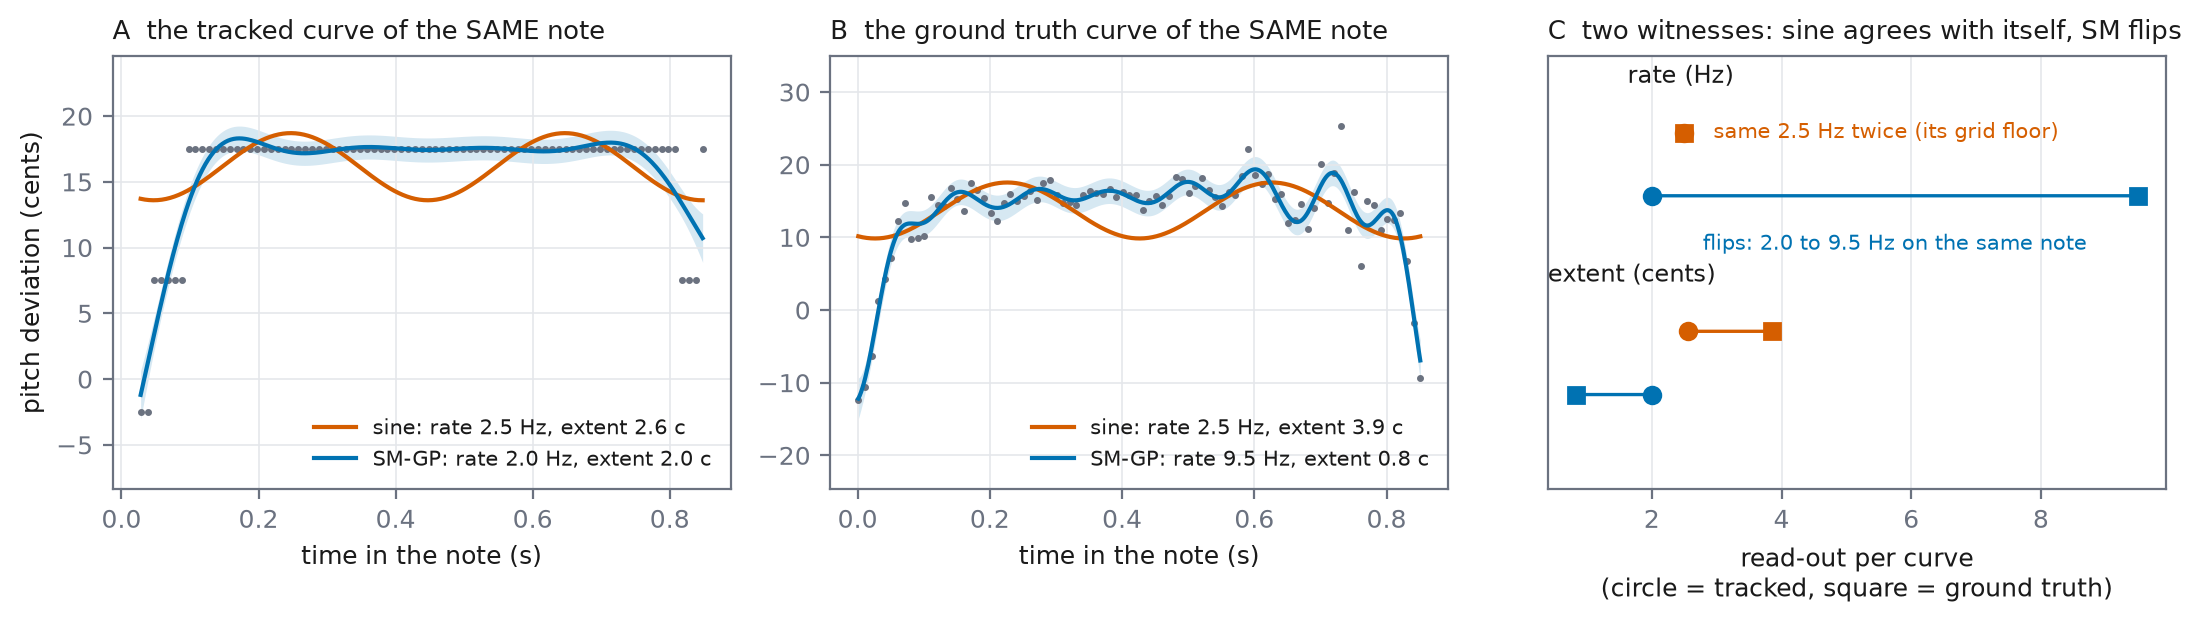
\includegraphics[width=0.98\linewidth]{sm_estimator_worstcase.png}

  {\scriptsize\textcolor{muted}{A barely vibrated bass note, its two
  measurements. The flexible posterior answers each curve honestly and
  differently. The sine fit returns its own grid floor twice. This
  instability at the scalar read out, verified intrinsic on strongly
  vibrated notes, is why the swap is closed.}}
\end{frame}

% ------------------------------------------------------------ backup
\begin{frame}{Backup: what the spectral mixture estimator was}
  The note's cents curve as a GP draw, kernel = two damped cosines:
  \[ k(\tau) = w_1 e^{-2\pi^2 v_1 \tau^2} \cos(2\pi \mu_1 \tau)
     + w_2 e^{-2\pi^2 v_2 \tau^2} \]
  \begin{itemize}
    \item Read outs: rate $= \mu_1$, extent from the posterior vibrato
          component, centre as the realized average. Fit per note by the
          exact marginal likelihood (grid over $\mu_1$, then local
          optimization), with uncertainties from the evidence curvature.
    \item Implementation forced three estimand fixes: realized amplitude
          not ensemble power, realized centre not the process constant,
          and a coherence bound so the component is an oscillation.
    \item The committed test: both estimators on the tracked AND the
          ground truth curve of each note, each scored against its own
          ground truth output, 5{,}157 development notes, parameter
          accuracy as the pass or fail rule. Full record:
          results/sm\_estimator\_dev.md and the two page note
          docs/sm\_estimator\_note.pdf.
  \end{itemize}
\end{frame}

\begin{frame}{Backup: the timing tail, before and after}
  \centering
  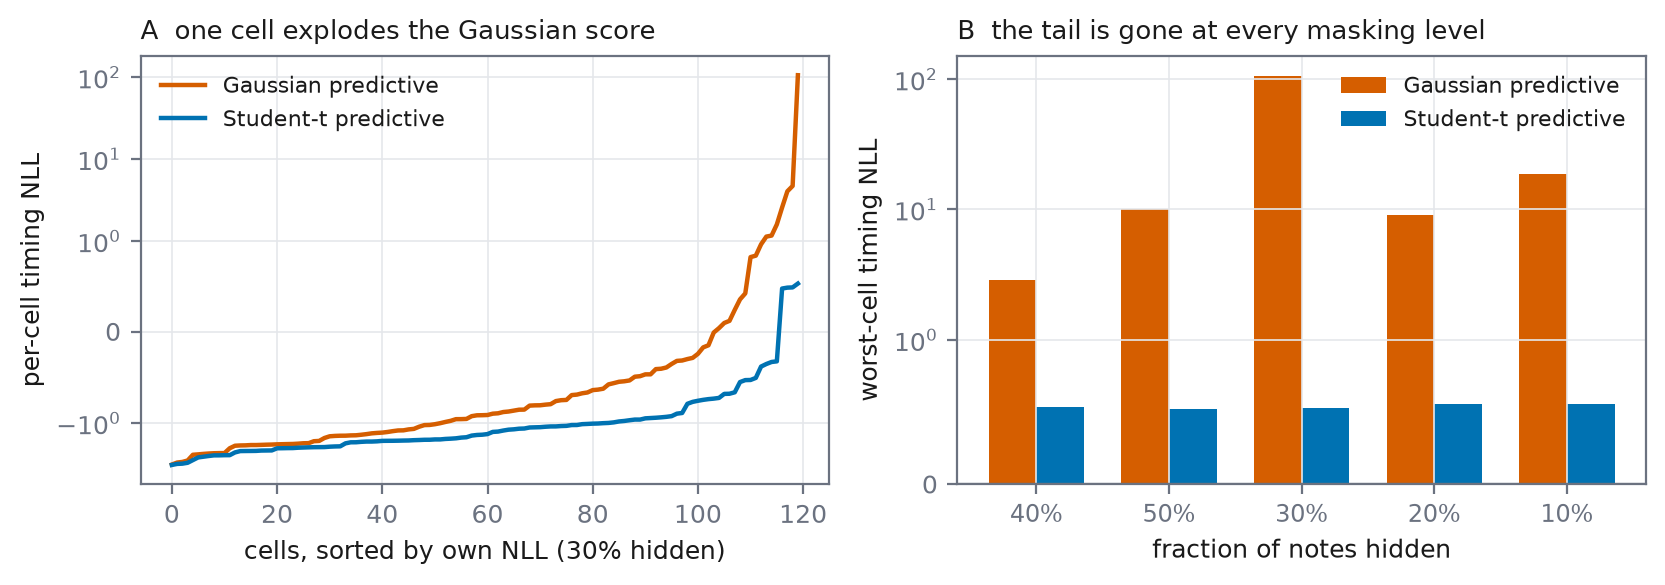
\includegraphics[width=0.92\linewidth]{tail_predictive_dev.png}
\end{frame}

\begin{frame}{Backup: robust timing noise helps articulation}
  \centering
  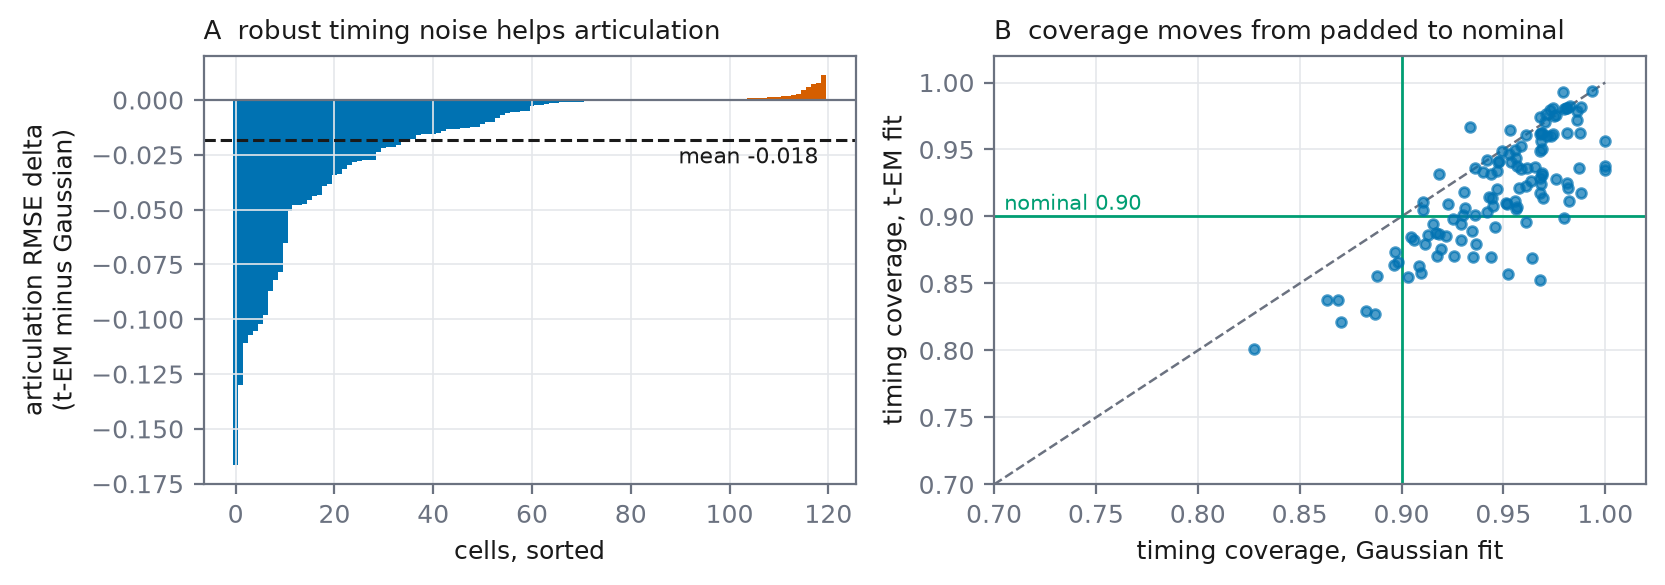
\includegraphics[width=0.92\linewidth]{t_noise_em_dev.png}
\end{frame}

\begin{frame}{Backup: the completion guard}
  \centering
  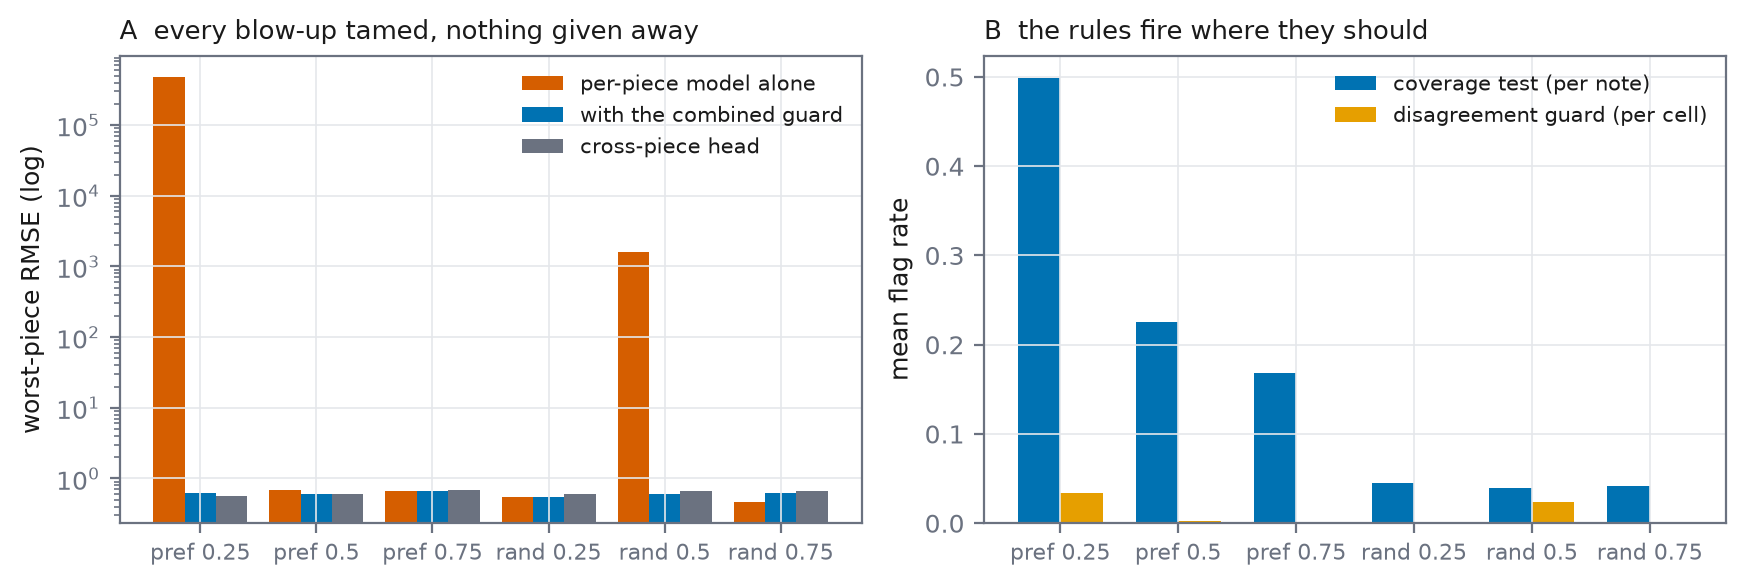
\includegraphics[width=0.95\linewidth]{completion_fallback_dev.png}
\end{frame}

\begin{frame}{Backup: the kernel question, closed in three panels}
  \centering
  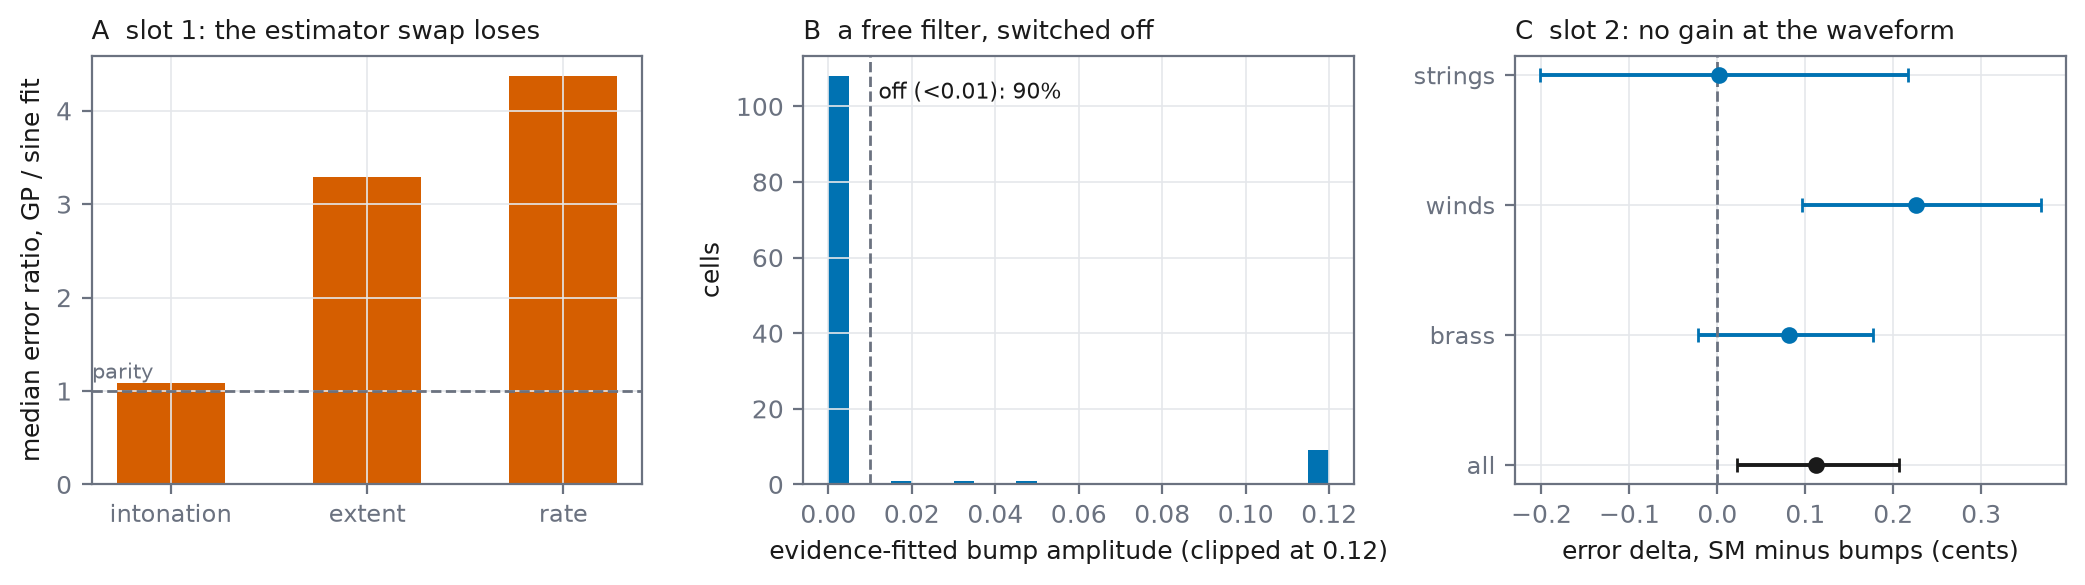
\includegraphics[width=0.98\linewidth]{kernels_closed_dev.png}
\end{frame}

\end{document}
